
\chapter{Open Virtual Platform Model and Multicore Debugging} % Main chapter title

\label{Chapter4} % For referencing the chapter elsewhere, use \ref{Chapter1} 

\lhead{Chapter 4. \emph{Virtual Platform Model and Multicore Debugging}} % This is for the header on each page - perhaps a shortened title

\section{Virtual Platform Overview}
Several important and interrelated trends in embedded systems that are forcing designers to reconsider basic issues of design and verification methodologies. Firstly, there is the emergence of distributed real-time applications running on integrated multicore platforms. Secondly, there is the necessity of hardware software co-design: the platform and application development must often take place in parallel. Thirdly, heterogeneous MPSoCs, systemswith different types of cores and hardware accelerators, provide a wide range of power and efficiency tradeoffs where the optimal mapping of application to resources must be aware of the platform resources. There is also the emerging area of reconfigurable computing where the hardware and software can adapt and reconfigure based on changing system state, thus adding an extra layer of flexibility and complexity to the picture of the heterogeneous platform.

The emergence of increasingly complex architectures makes testing and verification significantly more difficult. This is compounded by the need to be able to begin software verification prior to platform availability. Furthermore, the iterative design process can be more tightly executed when these stages are done in parallel. Often, many types of problems can be anticipated in early stages of design. It is easy to iamgine a situation where hardware is designed in isolation prior to software and problems are discovered during the early stages of software development that could easily be fixed by adjusting the hardware requirements. This cannot be done if they are developed in series since by that point the development of the hardware will be too far along to allow large structural changes. If they are designed in parallel, then optimal solutions that take into account both hardware and software adjustments can be considered and large trade-off decisions can be made with a fuller picture of the system in mind.

This has led to the development of increasing sophisticated and powerful platform simulation environments. Commercial products such as Imperas Multicore Development kit based off the Open Virtual Platform (OVP) standard as well as Mentor's Questa Multicore Simulator suggest that the debugging of distributed embedded software on virtual platforms is growing in popularity. 

With all that said, this project is much more modest in scope and may not have required platform virtualization if a team with more experience had tackled the software and hardware design in isolation. Being an inexperienced designer and having no background in formal testing or verification, it was very difficult to develop a comprehensive testing strategy for the hardware. This was very much an iterative learning process. The size of the project came to encompass both hardware and software. The possibility arose for bugs in the software or hardware in isolation, or due to a lack of understanding or foresight as to how the interface between hardware and software might behave. But there was no easy way to test the two halves of the problem in isolation, stimulating them with test vectors that approximated the other half. Quite a bit of progress was made over the first year, but quite a bit of time was also wasted. Confidence disappears and paranoia sets in when you are unsure if the current solution to the problem will work, even if executed perfectly. This lack of confidence can be a tremendous burden when strange behaviours are noticed in the system that can simultaneously arise from several bugs in the software and hardware as well as miscalculations in the initial conception. This is exacerbated by a lack of visibility into the system and no ability to isolate components and recreate system wide states. There's just a single ugly knot that needs untying and no obvious place to start loosening it.

\section{OVP Overview}

Platform virtualization with OVP provides several capabilities that have dramatically increased productivity when debugging new features since its development. The basic OVP workflow is shown in Figure \ref{f:ovp} Firstly, there is full system visibility. Breakpoints can be placed at any point in the code of any processor. Secondly, peripherals are treated as processor models. They are independent code threads activated by the simulator, meaning that they can also be debugged and breakpoints inserted in their functional model. Complex chains of events can be monitored automatically using scripts and full system visibility that are not possible when running on an FPGA. Full traces of all processors can be captured. Peripherals can be distilled to their most basic functional description while also presenting to the processors exact and identical control register interfaces. Code compiled using the Nios IDE given a QSYS generated platform specification runs with no modifications on the OVP platform derived from the same specifications. Functional verification of the hardware software interface can take place with much greater ease. Especially in the case where a bug arises out of an interaction between some software and hardware element, since in the virtual platform hardware is translated into software, it is much more easy to visualize, isolate, and remedy the problem.

\begin{figure}[h]
\centering
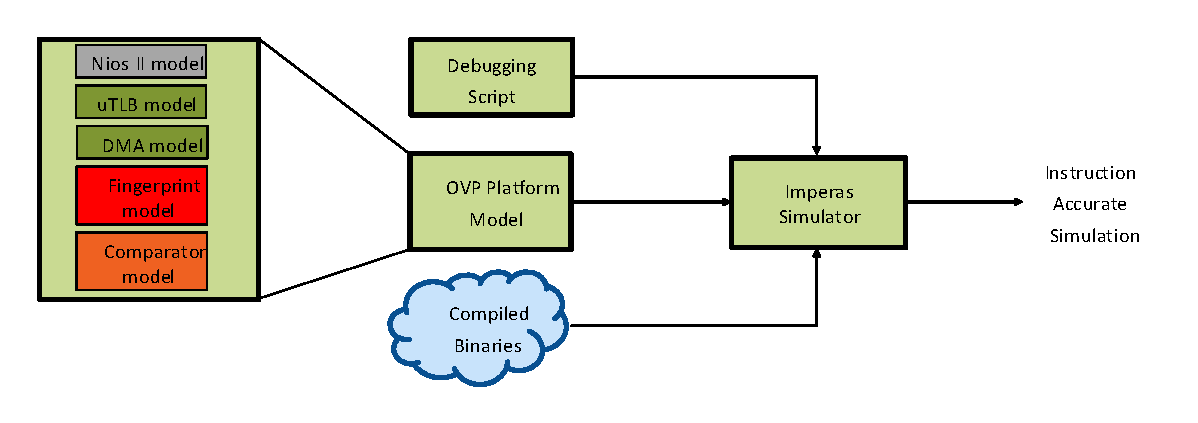
\includegraphics[scale=0.8]{Figures/ovp}
\caption{Platform virtualization workflow}
\label{f:ovp}
\end{figure}

\section{Processor Model}

The OVP processor model for the Nios II processor was co-developed with Altera and is fairly complete. Since the simulator is instruction accurate and does not take into account timing issues, the cache is omitted. Memory protection and memory management are available. One crucial aspect of the OVP system is that it is fully open source, allowing for modifications to the processor model to be made with relative ease. 

Fingerprinting involves a very strange type of peripheral that is concerned with all bus activity regardless of whether or not it is being addressed. Neither Quartus or OVP includes a built in mechanism for specifying a peripheral with this property. Therefore, it was note a trivial task to prepare the initial platform model that included a fingerprinting peripheral. 

The solution to the problem is ugly and is probably inefficient from a simulation speed perspective but it works and the technical details will now be discussed.

\subsection{Imperas Binary Intercept Technology}

In the OVP model, there are two types of behavioural descriptions: morph-time and run-time. The morph-time  API is used when creating a model description for the simulator to load the model. The run-time API is used to initiate behaviours while the simulator is running. Furthermore, there is a separate peripheral simulation engine (PSE). As it turns out, the processor simulation environment does not provide an easy way to do a seemingly simple thing. It is possible to add outgoing nets from a processor (although this is generally not done because the only outgoing signals from a processor should be the bus and buses have their own distinct model and port type). It is not possible to add to an instruction a command that stimulates one of these nets. 

Here is a more concrete example. The bus object in simulation is quite an abstraction and there is no way for a peripheral to see what is happening unless it is directly addressed. Therefore one solution is to add outgoing nets to the processor, and to modify the store instruction to stimulate those nets with information about the bus. The problem is that the code which defines the store instruction behaviour is considered morph-time by the simulator. Even if run-time APIs are included they will not be run after the simulation initializes. While it is possible to add nets to a processor, it is not possible for the processor to write values to those nets when executing store instructions. 

The Imperas Binary Intercept Technology (BIT) is a tool that allows additional run-time specifications to be added to a model as a separate shared library when the model is being loaded by the simulator. It is possible to use this tool to intercept and alter instructions as well as to monitor the system with complex chains of assertions. This is the API from which Imperas has developed their own prepackaged set of verification libraries (VAPs) and is therefore very powerful and able to reach deeply into the simulation environment.

The BIT provides two behaviours that allow the custom nets to convey information about writes. Firstly, it is possible to create a watchpoint over the entirety of memory for each core in the system. Whenever a write instruction is executed, this watchpoint is triggered. The callback of this watchpoint can then identify the processor that issues the instruction, as well as the address and data. It can then stimulate the nets associated with that processor such that they provide the information that a store has occurred as well as the address and data. These nets can then be directly connected to a fingerprinting peripheral. The BIT constructor and callback are shown in Listing \ref{l:vmi_callback}. Notice that the nets can carry 32 bit numbers, therefore three nets can carry all the information about a store instruction and that the run-time API (vmirt...) functions correctly.

\begin{lstlisting}[frame=single,language=C,label=l:vmi_callback,caption=VMI Memory watchpoint constructor and callback.]
//
// Constructor - install read and write callbacks on processor data domain
//
static VMIOS_CONSTRUCTOR_FN(constructor) {
    memDomainP domain   = vmirtGetProcessorPhysicalDataDomain(processor);
    Uns8       bits     = vmirtGetDomainAddressBits(domain);
    Addr       highAddr = (1ULL<<bits)) - 1;
    vmirtAddWriteCallback(domain, 0, 0, highAddr, writeCB, object);
}
static VMI_MEM_WATCH_FN(writeCB) {
    // we are interested only in writes made by processors (not artifacts of
    // simulation or memory accesses by other plugins, for example) so take
    // action only if processor is non null
    if(processor) {
        vmirtWriteNetPort(processor, vmirtGetNetPortHandle(processor, 
                "fprint_write_out_address"), address);
        vmirtWriteNetPort(processor, vmirtGetNetPortHandle(processor, 
                "fprint_write_out_data"), *((unsigned *)value));
        vmirtWriteNetPort(processor, vmirtGetNetPortHandle(processor, 
                "fprint_write_out"), 1);
    }
}
\end{lstlisting}

\section{Peripheral Models}
It was necessary to model the Altera provided DMA, mutex, as well as modify a prepackaged model of the Altera system timer. It was further necessary to model the comparator, the fingerprinting unit, the custom TLB, and the intercore IRQ bridge. The comparator and fingerprinting unit, including register sets, have been discussed already in some detail. This section will will give an overview of the DMA core and the TLB. The IRQ bridge is simply a bunch of register connected to the IRQ inputs of each core. Similarly the mutex is just a single register. All other functionality related to mutex behaviour is implemented in the sofware driver. Some simulation specific modifications will also be discussed.

\subsection{DMA}
A functional model of the DMA core was derived from the specification given in \cite{altera_ip_ug}. The timing characteristics of the DMA and any features related to packet size were omitted. The DMA peripheral therefore consists of one thread and one callback function that is triggered when the control register is written to by a processor. In line 4 of Listing \ref{l:dma}, the control register callback checks if the "GO" bit in the control register is written and if the length register has a non zero value (these functions should be self explanatory). If so, an event is triggered, causing the main DMA thread (line 21) to proceed past its wait condition. It should be fairly clear without any specific knowledge of the API that the main thread then updates its BUSY bit, performs the entire memory transaction in a single burst. Finally it updates all of its status bits. and notifies the processor with an interrupt if interrupts are enabled.

\begin{lstlisting}[frame=single,language=C,label=l:dma,caption=DMA model.]

PPM_REG_WRITE_CB(regWr) {
    *(Uns32*)user = data;
    if(DMACSP_ab8_data.control.bits.GO == 1 && DMACSP_ab8_data.length.value > 0){
        bhmTriggerEvent(start);
    }
}

static void dmaBurst(void) {   
    Uns32 len = DMACSP_ab8_data.length.value;
    char* buff = malloc(len);
    ppmReadAddressSpace (handles.MREAD,  DMACSP_ab8_data.readaddress.value, 
        len, buff);
    ppmWriteAddressSpace(handles.MWRITE, DMACSP_ab8_data.writeaddress.value, 
        len, buff);
    free(buff);
    DMACSP_ab8_data.length.value = 0;
    DMACSP_ab8_data.status.bits.LEN = 1;
}

static void channelThread(void *user)
{
    while(1) {
         bhmWaitEvent(start);
        
        //Start transaction
        DMACSP_ab8_data.status.bits.BUSY = 1;
         dmaBurst();
        DMACSP_ab8_data.status.bits.BUSY = 0;
        DMACSP_ab8_data.status.bits.DONE = 1;
        DMACSP_ab8_data.status.bits.REOP = 1;
        DMACSP_ab8_data.status.bits.WEOP = 1;
        if(DMACSP_ab8_data.control.bits.I_EN == 1){
            ppmWriteNet(handles.DMA_IRQ, 1);   
        }
    }
}
\end{lstlisting}

\subsection{TLB}
While the processor model comes equipped with an MMU, the translation process is completely transparent from the point of view of the intercept library and therefore there would be no easy way to integrate the TLB for fingerprinting purposes directly into the model. The same problem occurs with the actual HDL because the Nios core is encrypted. Keep in mind that for fingerprints to match, when main memory is used to store redundant state rather than dedicated scratchpads, the virtual address is required for fingerprint calculation.

The code for the TLB is a bit more cumbersome. It depends on a simulation object called a dynamic bridge that creates mappings from one address to another when a peripheral has both a master and slave port. An incoming address on the slave will continue on to the new translated address defined by the bridge. There is no thread or activity as with the DMA. There is no callback associated with the virtual address. There is no local memory object in the TLB associated with that address. The processor's fingerprinting nets are still activated by the intercept library. The TLB functions as follows:
\begin{itemize}
\item Wait until the TLB is enabled
\item Create a dynamic bridge for each translation entry in its table
\item Sort the table
\item Fill in the remainder of the address space with dynamic bridges that do not translate.
\end{itemize}

\section{Compensating for Simulation Artifacts}

The series of dynamic bridges breaks the intercept library to some extent. Simulation artifacts arise that cause fingerprints to stop matching. Both the physical and virtual address arrive at the fingerprinting unit, and sometimes several copies of them can arrive. Therefore, an interface between the TLB and fingerprinting unit must be added in order to allow the fingerprinting unit to know when translation is on and which addresses are being translated so that it ignores the physical addresses. Also, if the same data and address arrive twice in a row, it is assumed to be an artifact and is ignored. In the rare event where a program writes the same data to the same address on consecutive stores, the model simply falls a bit short in terms of its faithfulness to the physical platform. The model is very slow and running simulations in this fashion are not ideal for doing actual fault injection simulations. As a result, there is not much concern at the moment if an injected fault, once we begin developing OS services to replicate and restart threads, is masked on extremely rare events by this defective behaviour. 


\section{Case Study: Generated Code}
\label{s:matlabstudy}

\subsection{Fingerprinting a Simulink generated control loop}
Model based design is fundamental to automotive software engineering. An increasing proportion of the millions of lines of code that are currently used to run modern cars are computer generated \cite{mossinger2010software}. Furthermore, whether soft core or hard core, ISAs are established and compiler tool chains are mature and stable. One advantage of this architecture over single core hardening techniques is that no access or changes to existing core designs are required at the microarchitectural level. It is similarly advantageous to be able to leverage existing compiler and model-based code generation tools without requiring modifications. This second example demonstrates how fingerprinting can be used to monitor redundant executions of Simulink generated control code integrated into a simple RTOS template and compiled with \emph{gcc}.

Simulink Coder was used to extract transmission control logic from an example of an automotive drive train model \cite{sim_trans}. It would defeat the purpose and convenience of Coder to be forced to comb through and restructure the code to obey some style that is not natively supported. There are two things to note about the style of code: one that supports ease of fingerprinting and one that requires more attention. Firstly, the algorithm is a discrete FSM that will deterministically produce the same outputs given identical inputs. The tasks will match at the instruction level. The areas requiring more attention is the handling of global variables. Since the code will make hardwired references to global variables (i.e. the compiler will insert the absolute addresses into load and store instructions or calculate their position based on a global pointer register) it is necessary to ensure that separate duplicate copies are made for each core and that neither core is able to corrupt the original copy until fingerprinting is completed and the tasks are known to have been successful. 

Memory protection strategies is currently outside the scope of this work but the technology for implementing them is obviously well established. We assume that mechanisms are in place such that it is not physically possible for either plain core to write to the original data once a copy has been made. The final writeback must be done by reliable DMA initiated by a fault tolerant core (A core might be required to move the data out of the scratchpad to make room for another task or to provide a reference copy of data for rollback/reexecution purposes).

Once the global variables are copied into the scratchpads of the plain cores, memory translation is enabled to reroute references to global references away from main memory to the scratchpad. A full power MMU and OS virtualization services are not required. It is sufficient to ensure using linker options that the global variables are located in a contiguous block of data page aligned in accordance with the tag size of the uTLB and to annotate the global variables in the C code to be placed in the desired memory section. Meanwhile, the task stack must also be fit into the scratchpad and is accessed using its local physical address. As a further precaution, the global pointer register on each core are changed to match the GP register of whichever core the critical tasks were compiled for in case the compiler inserts GP relative address calculations. The context switch assembly code located in the BSP is then updated to include saving, resetting, and restoring the global pointer register so that any local interrupt handling code is not corrupted by a modified global pointer register should an interrupt occur during the critical task.